 \chapter{Giới thiệu đề tài}\label{chap:introduction}
	
	\section{Tổng quan đề tài}
	Nhu cầu vận chuyển hàng hóa đã có từ rất lâu. Cách thức vận chuyển hàng hóa phổ biến trước đây là thông qua đường bưu điện. Tuy vậy, trong thời đại 4.0 này thì hầu hết mọi dịch vụ đều đang được tự động hóa. Dịch vụ vận chuyển hàng hóa cũng không phải là ngoại lệ. Hiện nay có rất nhiều hệ thống vận chuyển hàng hóa đã được xây dựng. Chẳng hạn ở trong nước có thể kể đến Giao hàng nhanh, Giao hàng tiết kiệm vv... và ở ngoài nước là FedEx hay DHL. Những hệ thống hỗ trợ tự động hóa qui trình logistic và giao nhận hàng hóa là không ít. Tuy vậy việc có thêm một hệ thống sẽ giúp cho người dùng có nhiều lựa chọn để cân nhắc phù hợp với bản thân. Đặc biệt hệ thống nhóm xây dựng sẽ đào sâu hơn về quá trình vận chuyển hàng hóa
	\textbf{liên tỉnh}, tập trung vào những đơn hàng và kiện hàng có khối lượng lớn.\\
	
	Đề tài sẽ được thực hiện trên nền tảng web. Ứng dụng web app sẽ cung cấp các dịch vụ để quy trình vận chuyển hàng hóa liên tỉnh trở nên dễ dàng hơn cho người gửi/nhận, tài xế, thủ kho và quản lí.\\
	
	Ứng dụng sẽ bắt đầu từ việc người dùng gửi yêu cầu muốn giao món hàng bằng cách điền các thông tin cần thiết trên website hệ thống (Tên, địa chỉ bên gửi/nhận, chủ yếu bên nhận và bên gửi sẽ khác tỉnh và cách nhau xa). Sau đó, tài xế sẽ được hệ thống phân công đến những nơi lấy hàng theo yêu cầu bên gửi và tiến hành đi lấy hàng đến khi đầy xe.\\
	
	Sau đó, tài xế sẽ trở lại kho tập trung và gỡ hàng ra đặt trong kho. Quá trình này sẽ được lặp lại cho đến khi tổng hàng hóa thu gom về kho có thể chất đầy một xe container để tiến hành vận chuyển những kiện hàng đó đi liên tỉnh. Xe container đấy sẽ đi xuyên tỉnh và đến kho tập trung ở tỉnh ấy, gỡ hàng ra và sẽ có xe nội thành chuyển trực tiếp đến người nhận theo yêu cầu. Bên liên quan trong từng giai đoạn sẽ trực tiếp cập nhật tình trạng của đơn hàng để người dùng có thể lấy mã đơn hàng và xem trạng thái hiện tại của nó (Đang chờ, đang giao hàng, hoàn thành, etc.). Mỗi khi hàng được chuyển giao đều sẽ có biên bản giao nhận hàng được tạo ra cho mỗi bên.
	
	\begin{figure}[H]
		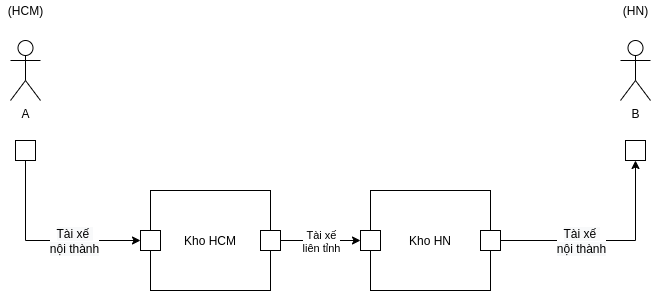
\includegraphics[width=1\textwidth]{/Summary.png}
		\centering
		\linebreak
		\caption{Luồng cơ bản giao nhận hàng hóa}
	\end{figure}
	
	
	\section{Mục tiêu và phạm vi đề tài}
	    Mục tiêu của đề tài là xây dựng một hệ thống vận chuyển hàng hóa liên tỉnh một cách có hiệu quả, giảm thiểu tối đa các sai sót có thể xảy ra trong quá trình giao nhận hàng hóa, cung cấp cho người dùng, tài xế, thủ kho, quản lý một giao diện trực quan, sinh động, dễ tương tác, giúp cho việc đặt hàng, nhận hàng, quản lý trở nên đơn giản và tin cậy hơn. Người dùng có thể tạo đơn hàng một cách rất dễ dàng và nhanh chóng. Hệ thống cho phép người dùng có nhiều lựa chọn về việc tự vận chuyển hàng đến kho hay nhân viên bên kho sẽ đến lấy nhằm giảm thiểu tối đa khó khăn khi vận chuyển một lượng hàng hóa lớn của người dùng. Sau khi đặt hàng người dùng có thể dễ dàng theo dõi quá trình hàng hóa được vận chuyển như thế nào, đã đến đâu, được vận chuyển bởi ai. Ngoài ra hệ thống còn tự động gửi thông báo qua mail để người dùng có thể biết chính xác trạng thái đơn hàng của mình. Hệ thống tích hợp chức năng thanh toán, giúp người dùng có thể theo dõi các đơn hàng đã hoàn thành và dễ dàng thanh toán qua các kênh trung gian như ZaloPay, Momo chỉ bằng một vài thao tác đơn giản. Tài xế có thể dễ dàng nhận đơn thông qua ứng dụng, quản lý các đơn hàng đang vận chuyển một cách tiện lợi, nhanh chóng. Từ lâu, việc quản lý đơn hàng, tài xế, phiếu xuất kho cũng là một vấn đề khá khó khăn, thì giờ đây hệ thống cung cấp khả năng lưu trữ tin cậy, đồng thời việc tìm kiếm rất nhanh, biểu đồ thống kê trực quan sinh động giúp cho nhân viên quản lý có thể dễ dàng theo dõi quá trình hoạt động của doanh nghiệp để có thể đưa ra các thay đổi, điều chỉnh khi cần thiết.
	    Việc xây dựng một hệ thống quản lý vận chuyển hàng hóa liên tỉnh như vậy đặt ra một số bài toán cần phải giải quyết như:
	    \begin{itemize}
                \item Công nghệ sử dụng là gì?
                \item Kiến trúc hệ thống như thế nào để có thể dễ dàng mở rộng khi có nhu cầu?
                \item Tổ chức lưu trữ dữ liệu thế nào để có thể truy xuất nhanh chóng, tránh làm ảnh hưởng không tốt đến trải nghiệm của người dùng? 
                \item Quá trình giao nhận hàng hóa của tài xế với người dùng hay của tài xế đối với thủ kho làm thế nào để quản lý và lưu trữ hiệu quả, tránh làm mất dữ liệu về sau?
                \item Việc phân phối đơn hàng cho tài xế đi giao/lấy làm thế nào để hạn chế tối đa chi phí bỏ ra cho doanh nghiệp cũng như người dùng?
                \item Làm thế nào để hệ thống có thể chịu tải cao, có thể xử lý lượng lớn các request đồng thời? 
                \item Làm thế nào để xác định được con đường vận chuyển giữa kho nguồn - kho đích là ngắn nhất để giảm thiểu chi phí? 
                \item Bảo mật cho ứng dụng cũng như xác thực người dùng như thế nào cho hiệu quả?
            \end{itemize}
	    
	
	\section{Cấu trúc luận văn}
	 
	 Phần còn lại của luận văn sẽ được tổ chức như sau:
	 \begin{itemize}
                \item Chương 2: Trình bày cơ sở lý thuyết về các công nghệ sử dụng
                \item Chương 3: Nói về các ứng dụng đã có và các nghiên cứu liên quan
                \item Chương 4: Nêu ra các bài toán và cách giải quyết cho từng bài toán
                \item Chương 5: Trình bày kiến trúc, đặc tả các chức năng, thiết kế cơ sở dữ liệu cho hệ thống
                \item Chương 6: Trình bày chi tiết về hiện thực hệ thống và kết quả đạt được
                \item Chương 7: Trình bày kết quả kiểm thử hệ thống
                \item Chương 8: Tổng kết, đánh giá kết quả
            \end{itemize}